\documentclass[journal]{IEEEtran} % use the `journal` option for ITherm conference style
\IEEEoverridecommandlockouts
% The preceding line is only needed to identify funding in the first footnote. If that is unneeded, please comment it out.
\usepackage{cite}
\usepackage{amsmath,amssymb,amsfonts}
\usepackage{algorithmic}
\usepackage{graphicx}
\usepackage{textcomp}
\usepackage{xcolor}
\usepackage{float}
\usepackage[justification=centering]{caption}
\raggedbottom

\def\BibTeX{{\rm B\kern-.05em{\sc i\kern-.025em b}\kern-.08em
    T\kern-.1667em\lower.7ex\hbox{E}\kern-.125emX}}
\newcommand{\imagewidth}{0.45\textwidth}
% \newcommand{\imageheight}{75mm}
\newcommand{\elvis}{\textit{Elvis}}
\begin{document}

\title{\elvis{}: A Highly Scalable Virtual Internet Simulator\\}

\author{%%%% author names
    \IEEEauthorblockN{Tim Harding},
    \IEEEauthorblockN{Jacob Hollands},
    \IEEEauthorblockN{Mitchell Thompson},
    \IEEEauthorblockN{Logan Giddings},
    \IEEEauthorblockN{Robin Preble},
    \IEEEauthorblockN{See-Mong Tan}
    \\%%%% author affiliations
    \IEEEauthorblockA{\textit{Western Washington University}}\\% first affiliation
    \IEEEauthorblockA{hardint, hollanj9, thomp288, giddinl2, prebler, see-mong.tan@wwu.edu}
}

\maketitle

\begin{abstract}
\elvis{} is a highly-scalable virtual Internet simulator that can simulate up to a hundred thousand networked machines communicating over TCP/IP on a single off-the-shelf desktop computer. This paper describes the construction of \elvis{} in Rust, a new memory-safe systems programming language, and the design patterns that enabled us to reach our scalability targets.  Traffic in the simulation is generated from models based on user behavior research and profiling of large web servers. We also designed a Network Description Language (NDL) to describe large Internet simulations.
\end{abstract}

\begin{IEEEkeywords}
    Virtual Internet Simulator, Rust, Network Description Language
\end{IEEEkeywords}

\section{Introduction}
\elvis{} is a highly scalable simulation of a virtual Internet. It runs cross-platform on Linux, Mac, and Windows computers, and is shown to accommodate simulations of more than twenty thousand machines sending and receiving TCP and UDP traffic on a standard, off-the-shelf Linux workstation.

\elvis{} is intended as a research tool, both for developing new networking protocols and for evaluating those protocols in a large network. It is also intended as a pedagogical tool for students to explore networking scenarios that are infeasible to realize without simulation, such as Distributed Denial of Service (DDOS) attacks.

\elvis{} is written in Rust\cite{rust}, a memory-safe systems programming language. We used \elvis{} to explore how Rust can simplify the development of systems software. We explore the software frameworks and design patterns required to construct very large scale simulations. Some key design choices are relying on language constructs for protocol stack isolation rather than OS-level virtualization, true zero copy of memory data throughout the simulation, as well as predicating concurrency on lightweight user-level coroutines rather than kernel threads. We also developed a Network Description Language that allowed us to specify very large simulations.

\section{Related Work}

The x-Kernel was an early approach to network simulation\cite{xk}. The x-Kernel architecture exemplified a highly-modular approach to implementing networking protocols in operating systems. Later work extended this into running the x-Kernel as a simulation. However, the goal was more focused on simulations to test protocol implementations rather than large scale simulations of an Internet.

Many commercial programs exist that allow users to construct simulated networks and learn how to configure network devices from different manufacturers. For example, the Cisco Packet Tracer provides a drag-and-drop interface to create networks of Cisco-specific devices [3]. Simulation sizes are typically small, on the order of tens of machines.

A common approach of researching internet simulators is to use OS mechanisms to isolate network stacks. For example, the Common Open Research Emulator (CORE) \cite{core} uses FreeBSD OS support to virtualize the kernel network structures that run in separate virtualized jails.  CORE reaches scales of a hundred virtual machines on one desktop computer.

A further example is the SEED Internet Emulator [5],  a Python library that implements autonomous systems and routers, including protocols like BGP. The system is geared toward cybersecurity pedagogy and allows users to set up a virtual Internet that can be used to emulate scenarios like BGP poisoning or blockchain attacks. SEED is based on Docker\cite{docker} containers to provide isolation between machines in the simulation.

\elvis{} differs from previous work in that high scalability is a primary goal of the simulation. In one experiment wherein many machines send a single UDP message to a single receiver, we were able to scale up to more than 100,000 machines. In a separate experiment where all machines in the simulation continuously and concurrently send and receive data, we were able to scale up to 20,000 machines in a single simulation before memory limits were encountered. \elvis{} also provides ground-up, parallelizable constructions of key protocols including TCP/IP, DNS, and DHCP. rather than rely on existing OS implementations and virtualization technologies for isolation between machines. Instead, \elvis{} runs entirely in user space, vastly reducing both memory usage and overhead due to context switches. Concurrency is achieved with the Tokio\cite{tokio} lightweight coroutine library.

\section{Rust}

Rust is a general purpose programming language that is focused on performance and memory-safety. Unlike languages like Java or C\# that maintain memory-safety with a garbage collector, Rust maintains memory-safety by requiring that all references point to valid memory through the use of the compiler.

Memory in Rust is reclaimed when owning variables go out of scope. The potent result of this is that a Rust program that compiles has a much lower risk of leaking memory,  and also guaranteed to never have a segmentation fault due to the invalid access of memory. Without a garbage collector, Rust is also as fast as C or C++\cite{rust-speed}.


\subsection{Rust and Memory Safety}

The Rust borrow checker tracks the lifetimes of pointers, making sure that all references are valid and a heap allocation is not freed until all references are released.

Only one variable can ``own'' a pointer. Assigning the pointer to another variable transfers ownership of the pointer, and the pointer can no longer be accessed with the original variable. This is conceptually similar to C++'s unique\_ptr smart pointer, but Rust enforces this strictly at compile time. Temporary references to a pointer may be passed to functions to use, but the compiler ensures that the lifetimes of those references never exceed the lifetime of the owning variable. When the owning variable goes out of scope, the memory that the pointer references is freed.

In situations where it is critical for multiple references to exist for shared data, Rust provides reference counted smart pointers Rc$<$T$>$ (reference counted pointers of type T). For reference counted pointers that work across threads, Rust provides Arc$<$T$>$ (atomically reference counted pointers of type T). \elvis{} makes liberal use of these language features.

\subsection{Unsafe Rust}

Programmers can circumvent Rust's memory-safety by marking a region of code ``unsafe''. This is usually needed when Rust calls into C-code, which is by nature unsafe. The onus is on the programmer to make sure that memory safety is preserved in unsafe Rust code.

\elvis{} makes no use of unsafe Rust. Memory-safety is maintained throughout the simulation.

\subsection{Concurrency}

Rust provides native support for concurrency through the thread:: module. In Unix, this is a wrapper on top of POSIX threads.

We chose instead to base our implementation on the Tokio \cite{b6} library. Tokio provides users with the ability for asynchronous programming using async/await functions. More important to \elvis{}, Tokio allows user level coroutines to be multiplexed on top of kernel threads.
Coroutine resource usage is significantly lower than threads that require both a
user-level stack as well as a kernel-level stack.

\subsection{Trade Offs}

The drawback to Rust is that the programming paradigm requires a much steeper learning curve. Programmers new to Rust often report ``fighting the borrow checker''. This situation improves with experience but is certainly a real impediment. In our experience, students new to the \elvis{} research group typically spend one academic quarter simply becoming comfortable
with Rust.

\section{Architecture}

\subsection{\elvis{} Core}

The two main constructs in \elvis{} are machines and networks. Machines model some device running an operating system, such as a computer or smartphone. Each machine is modeled after the x-Kernel design. A machine is a container for a set of protocol objects which interact with one another through an abstract interface. Some standard protocols that are included in most machines are IPv4, UDP, and TCP. User applications such as client and server programs are also modeled as protocols for uniformity. Each protocol can create sessions, which are objects that represent a particular network connection. Sessions are created either when an upstream protocol makes an active open to a remote host or when a packet comes in for which there is no existing connection and an upstream protocol is listening, as in the case of server programs. Sessions form a chain with each contributing protocol providing a link.

\begin{figure}[htbp]
    \centerline{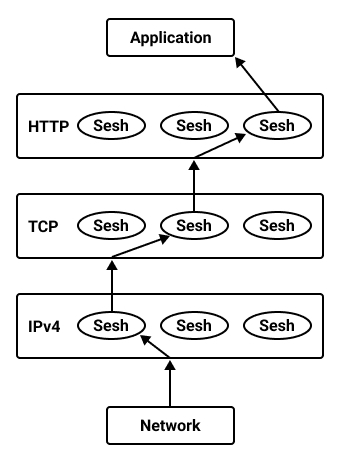
\includegraphics[height=6cm,keepaspectratio]{Images/Demux.jpg}
    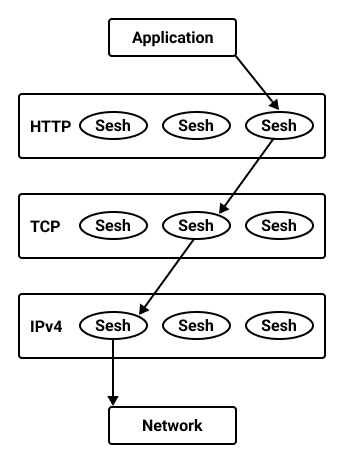
\includegraphics[height=6cm,keepaspectratio]{Images/Send.jpg}}
    \caption{Receive and send paths in x-Kernel protocol graph.}
    \label{fig:xkernel}
\end{figure}

For example, a user application may hold a TCP session which in turn holds an IPv4 session. Sessions take charge of sending packets by appending headers and forwarding the packets to downstream sessions, while protocols receive incoming packets and decide which session to demux each packet to based on network headers.

Machines are connected to networks, which are the conduit through which packet traffic passes. Networks are designed to abstractly model a variety of real-world networking technologies, such as Ethernet, Wi-Fi, and point-to-point communication. To simulate a variety of underlying technology, networks can be configured with different throughput, latency, packet loss, and packet corruption characteristics. In this way, \elvis{} models networking down to the data link layer. In keeping with our focus on large-scale simulation, we choose to omit the details of any particular physical networking protocol for the sake of performance and uniformity. Instead, an \elvis{} network provides functionality that is common to most data link protocols, such as unicast, multicast, broadcast, and standard frame header information such as MAC addresses.

In order to make our networking as efficient as possible, our simulation uses a bespoke message data structure that allows addition and removal of headers, slicing, and sharing without copying or moving bytes. This helps us avoid serialization and deserialization of network traffic for efficiency gains. All of our protocols are written from scratch to take advantage of this data structure. For example, where most TCP implementations expect flat byte arrays for input and copy segment text into ring buffers, our implementation uses zero-copy concatenation of messages and accesses bytes through an iterator interface to circumvent the need for serialization.

With this model, we are able to isolate machines from one another without heavy-duty mechanisms such as containers. Instead, we use asynchronous functions to deliver packets over networks and avoid context switches. Because of Rust’s guarantees, users need not worry that unsafe memory accesses will break isolation such that a malfunction in one machine can affect another.


\subsection{Network Description Language}

Previously, simulations in \elvis{} required a great deal of manual setup using Rust. The solution to this was a Network Description Language (NDL) to allow for not only easier setup, but also for the possibility of large scale simulations.

Using Rust to define these simulations would cause core problems for users for two main reasons. First, not all end users will be fluent in Rust, and due to the intricacies of how simulations must be defined this is a major limiting factor. A user would have to manually define each part of the simulation in Rust and be familiar with each part of \elvis{} in order to do so. Second, large scale simulations would not be impossible to define, but tremendously difficult and time consuming. Each machine, and application written out and defined in Rust would mean some of the larger scale simulations would need hundreds if not thousands of lines of code just to be run. Our NDL simplifies the process of programming by enabling the creation of easily definable and reproducible sections. This, in turn, facilitates the rapid development of large-scale simulations.

Typical NDLs use a variety of different languages to define their protocols. Some choices initially considered were XML and JSON, however given the idea of protocols being contained within parts of the simulations we decided to create a language using tabbed blocks. This allows nesting of sub protocols and definitions within other sections, and allows for repeatability of these sections.

To define a simulation, two core components are required: a set of Networks and a set of Machines. Within those there can be as  many Network and Machine sections as needed. Each Network can currently contain either statically defined single IPs or a range of IPs. As many single IPs or range of IPs may be defined in the Network sections. Following that pattern, a Machine will contain a similar structure. Each Machine must contain Protocols, Applications, and Networks. These three components help clearly define the location and function that the Machine will serve. Protocols such as UDP or TCP may be used, a set of Applications such as sending or receiving messages may be used, and finally a set of Networks the machine is on must be defined. See Figure \ref{fig:basic} for an example of the NDL.

\begin{figure}[htbp]
    \centerline{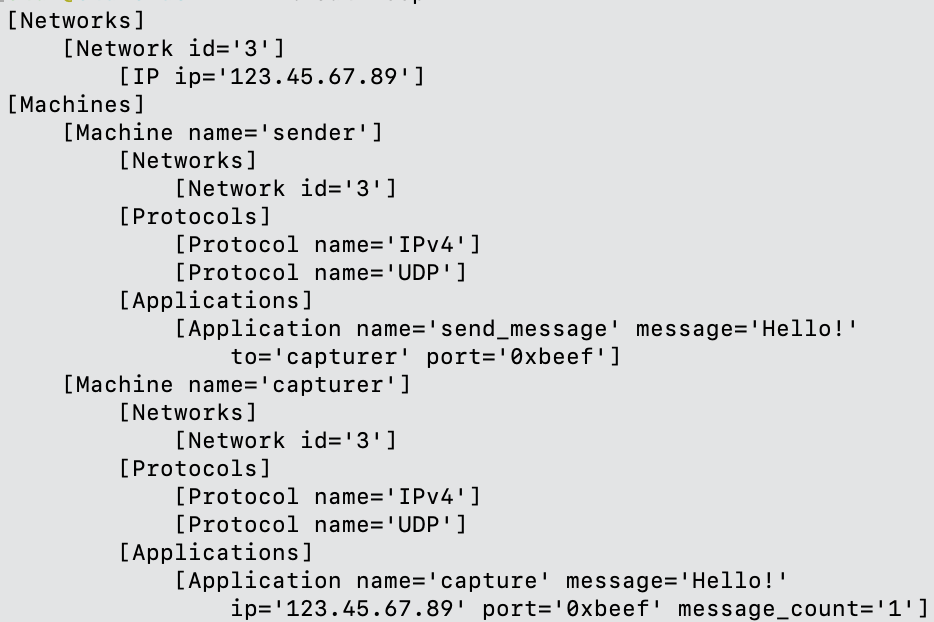
\includegraphics[width=\columnwidth]{Images/ndl-sample-new.png}}
    \caption{Basic example simulation.}
    \label{fig:basic}
\end{figure}

Each of those sections are defined using a tabbed structure. A core declaration will be tabbed zero times, a sub declaration one time, and so on. For example, a Networks section will be at zero tabs, a Network defined in that section will be at one tab, and each IP definition for that Network will be tabbed twice.

Arguments for subsections can be defined freely. Other than the core needs of a specific application or protocol, such as the name of the protocol or the IP range of a network, users can define any such argument needed and it will be read in. This argument then gets stored with the rest of the arguments, core or otherwise, and can be accessed in the generator code. Users have no extra steps in defining new applications or protocols for use other than adding checks for those new applications or arguments, then accessing and using them.

Putting all of those sections together results in a complete language for defining in depth simulations for \elvis{}.

\subsection{Socket API}

One of our goals in designing \elvis{} was retaining the ability to easily port existing applications into the simulation. In order to achieve this, we needed a socket API that closely mimicked UNIX sockets, with functionality of creating sockets, using sockets to connect to a server machine or listen and accept incoming client connections, as well as sending and receiving messages over the network.

A challenge in doing this is the fact that the machines in \elvis{} operate using a x-Kernel style protocol stack, which is incompatible with writing UNIX style applications.
The \elvis{} socket API serves as an interface between the two.
A second drawback is that UNIX style sockets have undesirable aspects to their implementation, such as  pointer casting.
\elvis{} presents a modernized  implementation while retaining all the functionality needed.

The resulting socket API is familiar and easy to use for anyone who has experience writing server-client applications using UNIX sockets, with the only noticeable differences being syntactical ones and the fact that applications utilizing it are written in Rust instead of C. This allows for convenient conversion and porting of existing UNIX server-client applications into \elvis{} applications.

Note that it is not the goal of \elvis{} to support full OS-level functionality in the
simulation. \elvis{} applications are limited to using the \elvis{} Socket API to
create network connections, and send/receive data.

\subsection{Web Traffic}

In order to create realistic simulations of the Internet within \elvis{}, we require realistic traffic. One primary category of traffic is web traffic between clients and servers.  To do this, we first have to characterize servers on the internet.

That means gathering data from top servers on the size, number of links, number of images, and the size of images for each page on a web server. The distribution of that  data will then be used to model the distribution of web pages on that type of website. Our simulated web servers will generate html pages for “users” to browse based on the distribution of size, number of links, and images sizes for that category of website.

We started by creating a web scraper in Rust that recursively traverses a website and outputs the links and images on each page as well as the size. We chose yahoo.com to test this scraper since it is a large site and most of the links on Yahoo lead to other pages on the site. We scraped over 200,000 pages.

When analyzed, we found that for each attribute measured, the majority of pages tended to fall within a narrow range of values with the rest being fairly scattered without a clear distribution. This made it difficult to find a simple mathematical model of the distribution. Instead, we created a program that went through the data for each page characteristic (size, number of links, etc.) and sorted it into buckets while keeping track of how many pages fell into each bucket. This information was saved in a .csv, which can then be passed into the web server program to inform the characteristics of the html pages it generates so the web server can mimic the servers we gathered data from.

\begin{figure}[htbp]
    \centerline{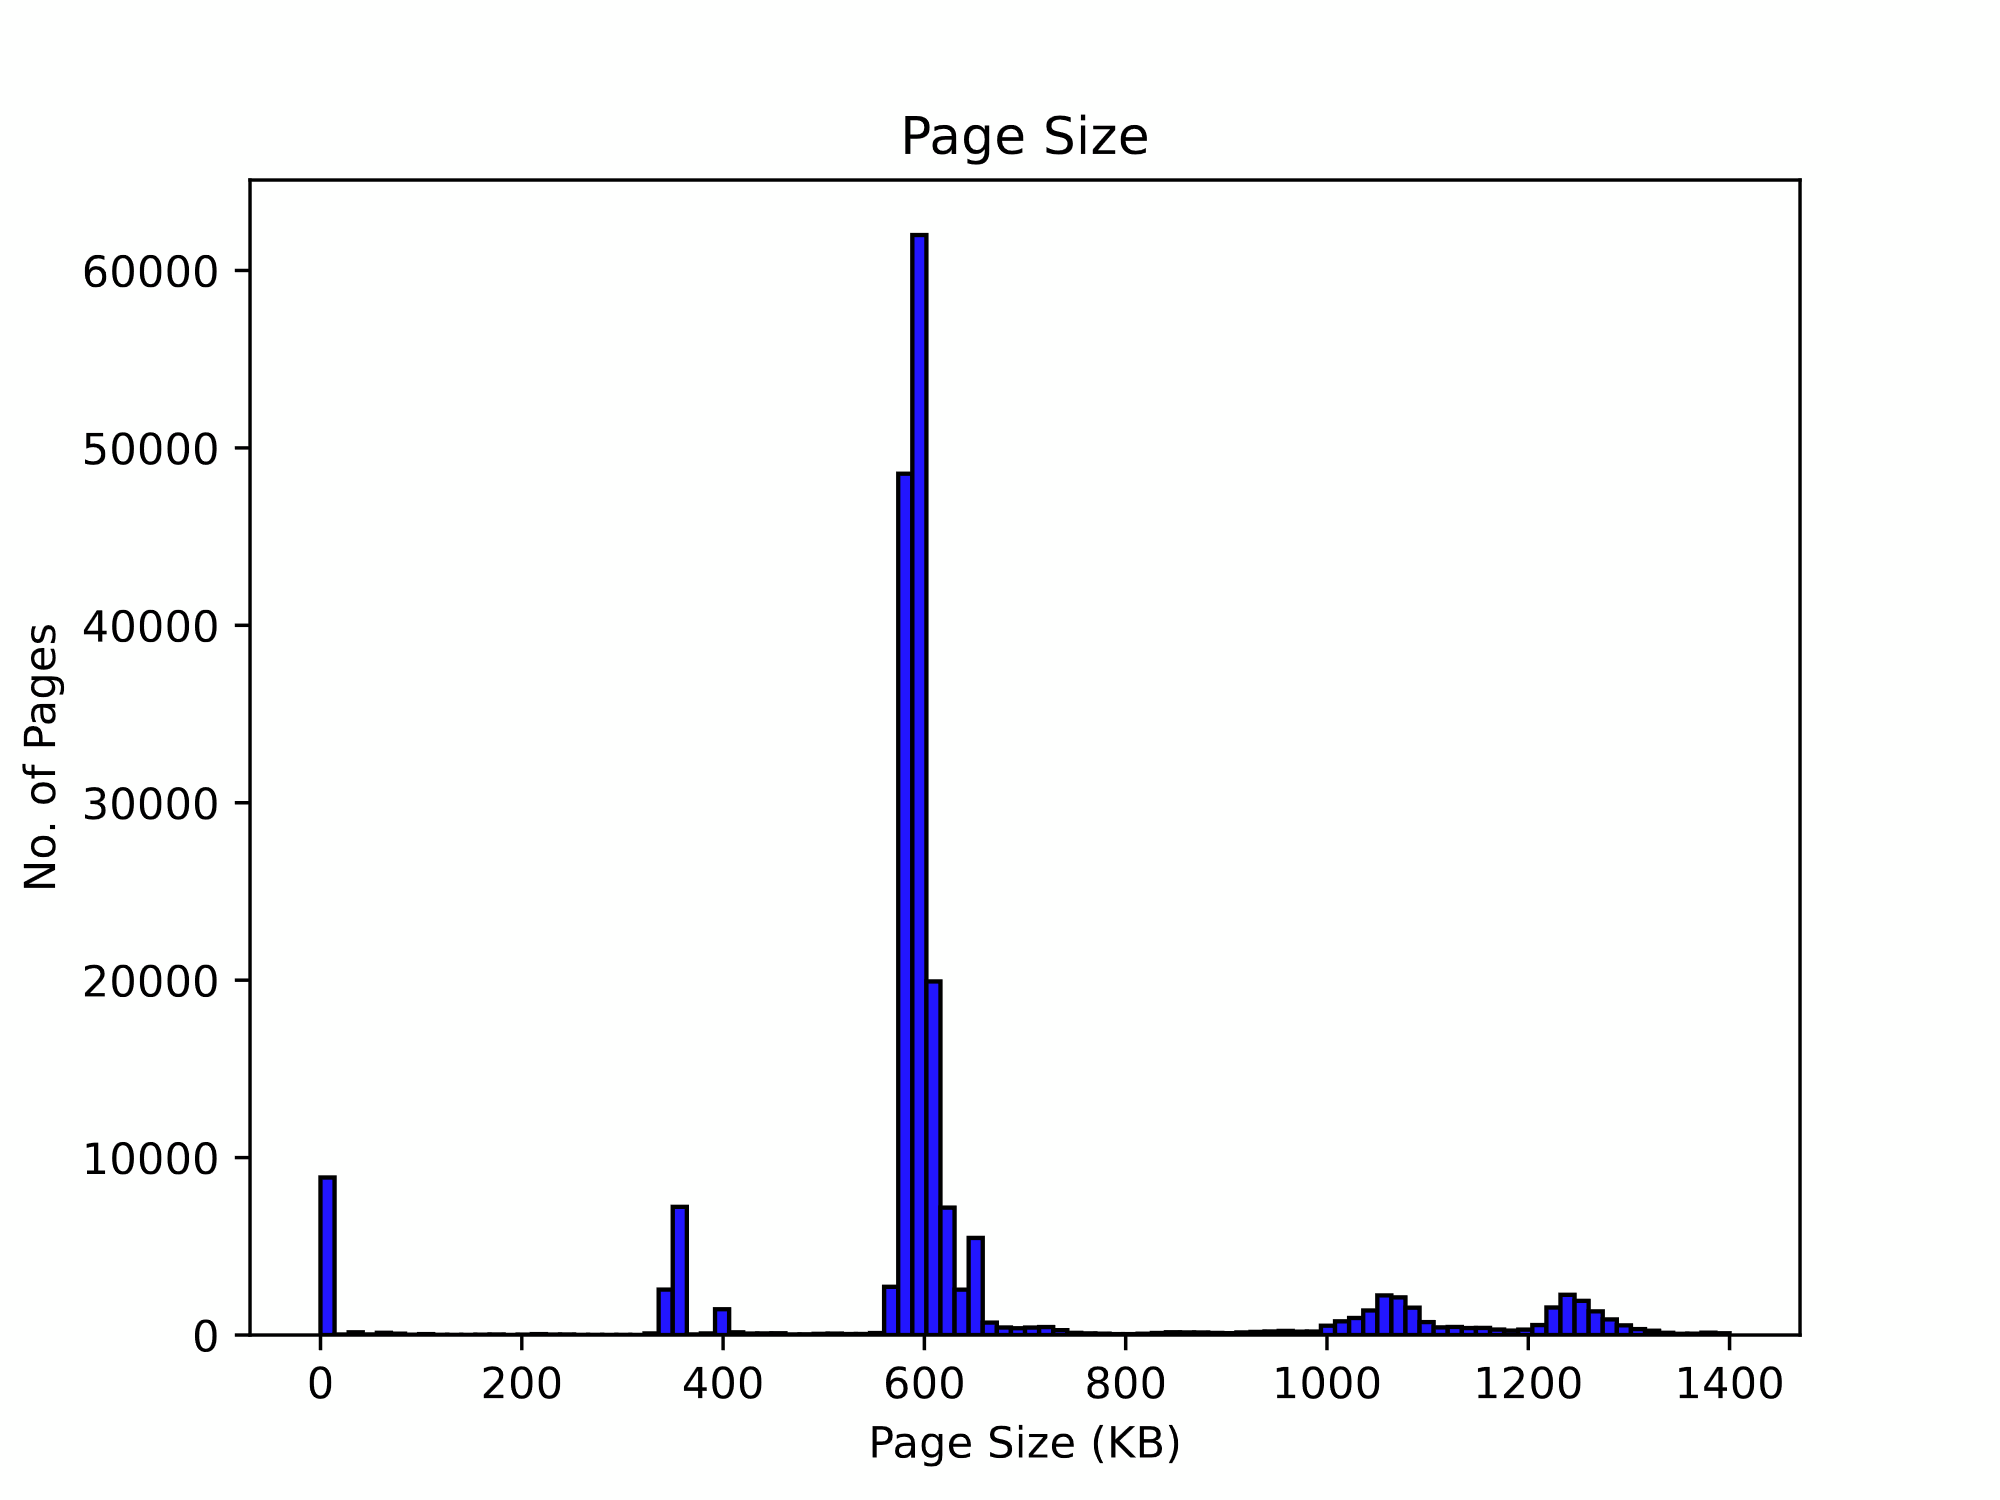
\includegraphics[width=\imagewidth]{Images/web_sizes.png}}
    \caption{Distribution of web page sizes on Yahoo.com.}
    \label{fig:websize}
\end{figure}

In further work, we developed an application that mimics how users typically behave when browsing web pages.

\section{Experimental Results}

\subsection{Scalability}

To test \elvis{}' scalability we ran a variety of simulations on two core simulation types. The two types used were a low bandwidth high machine count simulation, and a high bandwidth lower machine count simulation. The low bandwidth focuses on a higher machine count, but does not keep the machines running concurrently, meaning the machines send messages one at a time to keep overall system load low and simulates an environment where users could be connecting to a server and then disconnecting when they are done. The high bandwidth focuses on keeping the machines concurrent, leading to a lower overall machine count. This means that the machines are all trying to send their 1,000 messages at once to the server. This better simulates a massive load on \elvis{}.

To accomplish these simulations, a robust testing system was needed. We designed a Bash script and Python-based system that runs various simulations and tracks memory usage, CPU usage, and execution times of the simulations. This data is then compiled into JSON for storage which is then used to generate graphs automatically using Python’s MatPlotLib. Additionally, all the following tests were run on an Intel Core i5-8279U CPU, with 16 GB of RAM.

\subsubsection{Low Bandwidth Simulations}

The first set of simulations ran was to test \elvis{} capabilities with lots of machines all running at once. To do this the simulations were designed to generate a set amount of machines all sending a message to a single machine. That machine is then configured to receive that same amount of messages as the number of machines created. This was tested on machine counts ranging from one thousand to one million.

\begin{figure}[H]
    \centerline{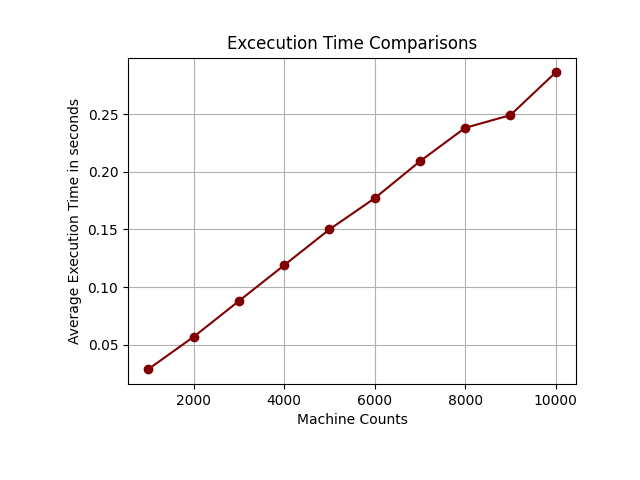
\includegraphics[width=\imagewidth]{Images/low_band_one_to_ten.png}}
    \caption{Execution times of low bandwidth simulation with machine counts from 1,000 to 10,000.}
    \label{fig:low_band_one_to_ten}
\end{figure}

\begin{figure}[H]
    \centerline{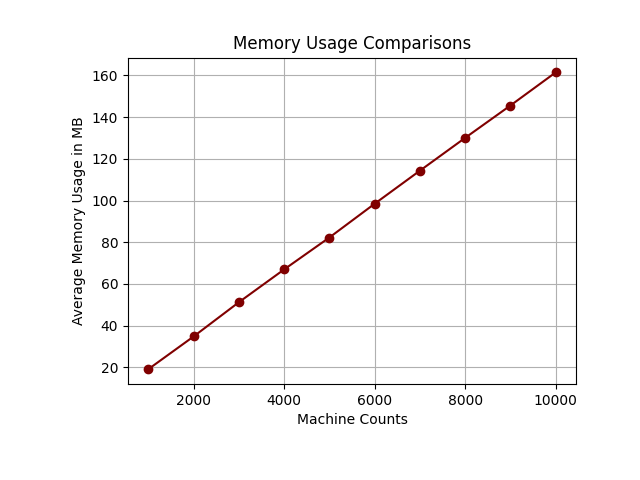
\includegraphics[width=\imagewidth]{Images/low_band_memory_one_to_ten.png}}
    \caption{Memory usage of low bandwidth simulation with machine counts from 1,000 to 10,000.}
    \label{fig:low_band_memory_one_to_ten}
\end{figure}

\begin{figure}[H]
    \centerline{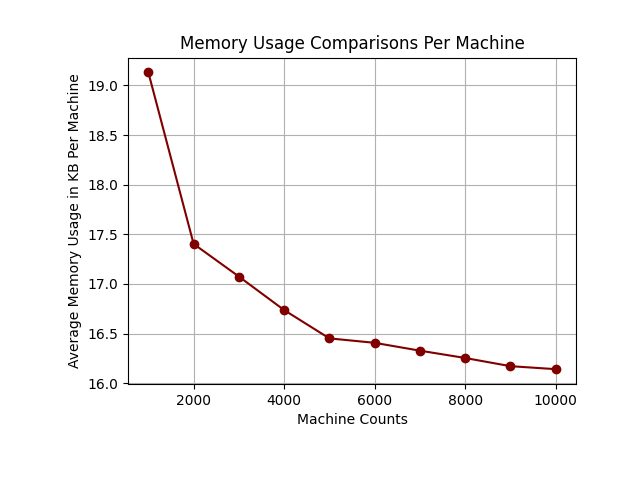
\includegraphics[width=\imagewidth]{Images/mem_usage_per_machine_thousand_to_ten_thousand.png}}
    \caption{Memory usage per machine of low bandwidth simulation with machine counts from 1,000 to 10,000.}
    \label{fig:low_band_memory_per_machine_one_to_ten}
\end{figure}

As seen in Figures \ref{fig:low_band_one_to_ten} through \ref{fig:low_band_memory_per_machine_one_to_ten}, low bandwidth simulations with 1,000 to 10,000 machines start to develop a distinct pattern. As machine count increases overall execution time and memory usage increases linearly. Memory usage per machine in the simulation decreases as the simulation's overhead is amortized over more machines. The average memory usage per simulated machine is slightly above 16 KB.

\begin{figure}[H]
    \centerline{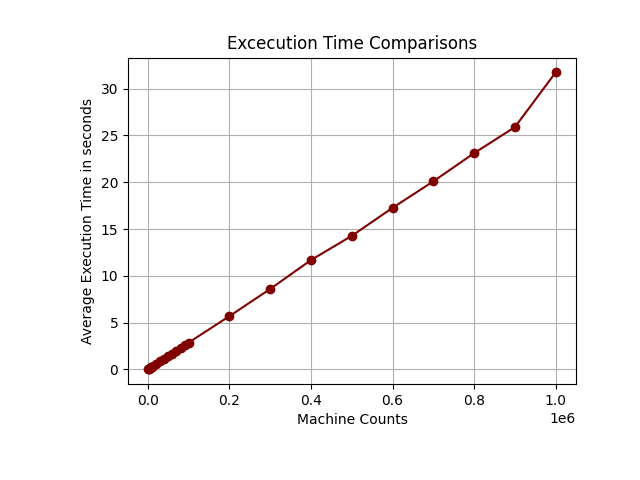
\includegraphics[width=\imagewidth]{Images/time_low_band_thousand_to_million.png}}
    \caption{Execution times of low bandwidth simulation with machine counts from 1,000 to 1,000,000.}
    \label{fig:low_band_one_to_million}
\end{figure}

\begin{figure}[H]
    \centerline{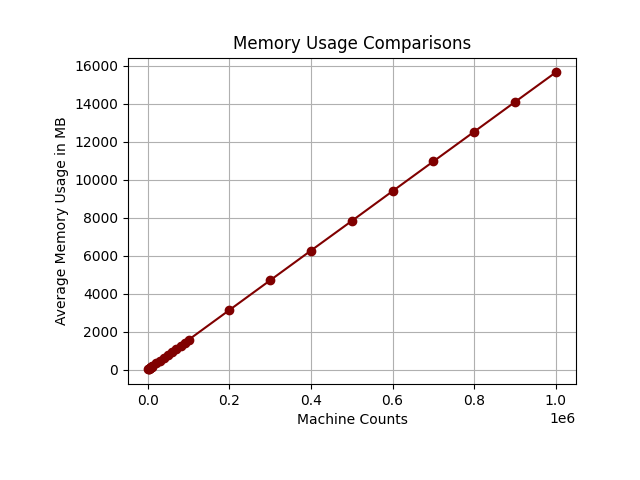
\includegraphics[width=\imagewidth]{Images/mem_usage_low_band.png}}
    \caption{Memory usage of low bandwidth simulation with machine counts from 1,000 to 1,000,000.}
    \label{fig:low_band_memory_one_to_million}
\end{figure}

\begin{figure}[H]
    \centerline{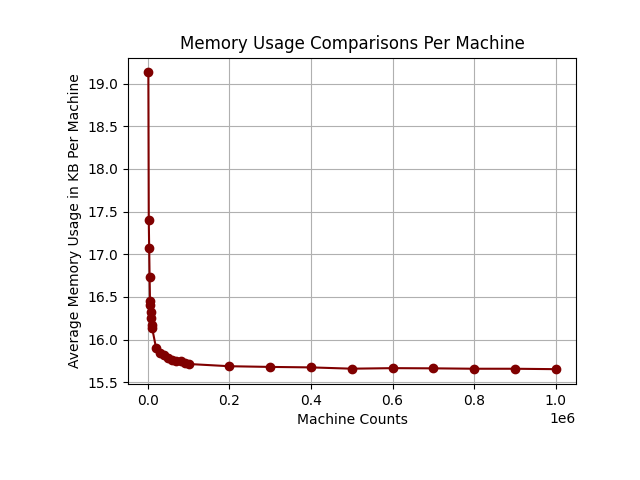
\includegraphics[width=\imagewidth]{Images/mem_usage_per_machine_low_band_thousand_to_million.png}}
    \caption{Memory usage per machine of low bandwidth simulation with machine counts from 1,000 to 1,000,000.}
    \label{fig:low_band_memory_per_machine_one_to_million}
\end{figure}

\begin{figure}[H]
    \centerline{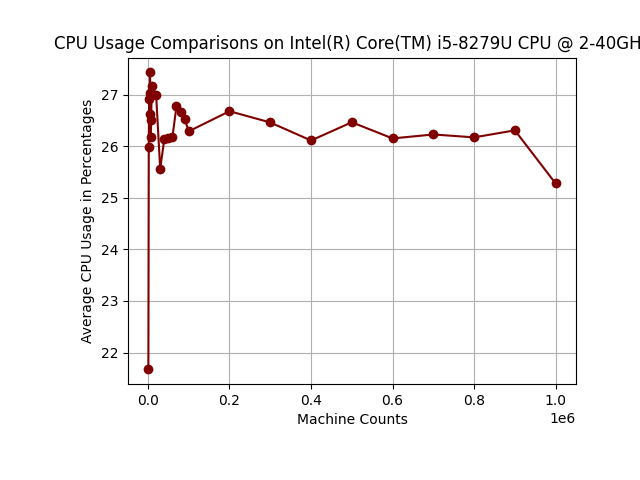
\includegraphics[width=\imagewidth]{Images/CPU_usage_low_band.png}}
    \caption{CPU usage of low bandwidth simulation with machine counts from 1,000 to 1,000,000.}
    \label{fig:low_band_cpu_one_to_million}
\end{figure}

In Figures \ref{fig:low_band_one_to_million} through \ref{fig:low_band_memory_per_machine_one_to_million} the previously noticed patterns become more prevalent. Once again, as machine count increases, overall execution time and memory usage increase linearly and memory usage per machine in the simulation decreases due to amortization of the core invariant simulation resources. One interesting part to notice is that machine specific memory usage plateaus as we approach the system's physical memory limit.

\subsubsection{High Bandwidth Simulations}
The next set of simulations ran was to test \elvis{} capabilities with lots of machines all running at once; however, each machine now sends 1000 messages. This means that the total count of messages sent is machine count multiplied by 1000 and it also means that each machine lives for longer within the simulation.. The goal with this was to generate machines in such a way that we could find the limits for concurrent full usage of \elvis{} rather than just the single message per machine case.

\begin{figure}[H]
    \centerline{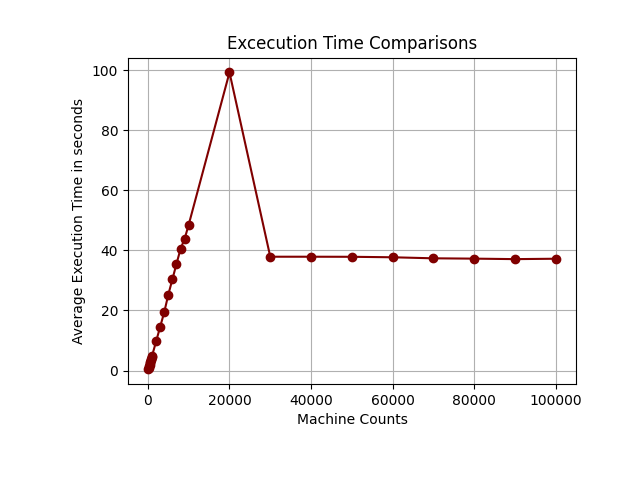
\includegraphics[width=\imagewidth]{Images/time_high_band.png}}
    \caption{Execution time of high bandwidth simulation with machine counts from 1,000 to 100,000}
    \label{fig:time_high_band}
\end{figure}

\begin{figure}[H]
    \centerline{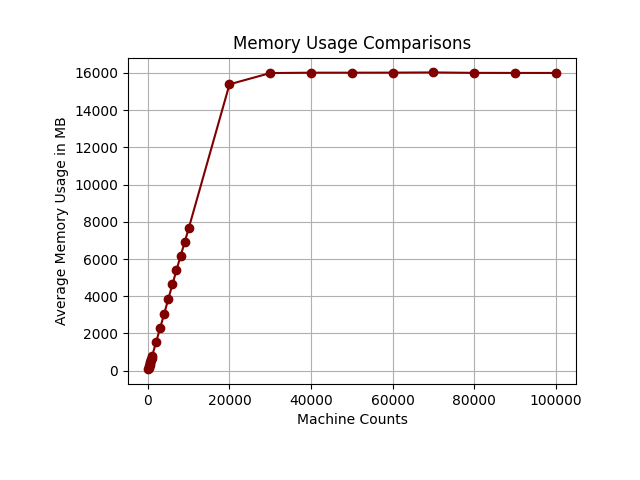
\includegraphics[width=\imagewidth]{Images/mem_usage_high_band.png}}
    \caption{Memory usage of high bandwidth simulation with machine counts from 1,000 to 100,000}
    \label{fig:mem_usage_per_machine_high_band_thousand_to_hundred_thousand}
\end{figure}

\begin{figure}[H]
    \centerline{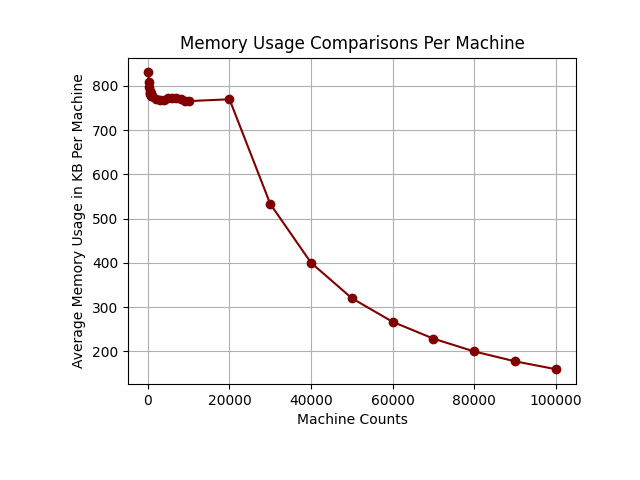
\includegraphics[width=\imagewidth]{Images/mem_usage_per_machine_high_band_thousand_to_hundred_thousand.png}}
    \caption{Memory Usage per machine of high bandwidth simulation with machine counts from 1,000 to 100,000}
    \label{fig:mem_usage_per_machine_high_band_thousand_to_hundred_thousand}
\end{figure}

\begin{figure}[H]
    \centerline{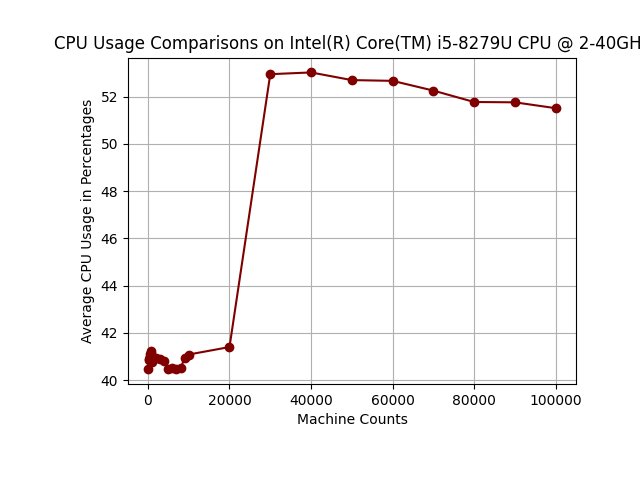
\includegraphics[width=\imagewidth]{Images/CPU_usage_high_band.png}}
    \caption{CPU usage of high bandwidth simulation with machine counts from 1,000 to 100,000}
    \label{fig:CPU_usage_high_band}
\end{figure}
% Fix the fig nums
In Figures \ref{fig:time_high_band} through \ref{fig:mem_usage_per_machine_high_band_thousand_to_hundred_thousand} the pattern differs from the low bandwidth tests in an interesting way. From 1,000 to 20,000 machines, it follows a similar linear pattern of growth. However, passing the 20,000 machine mark our system reaches the full usage of the 16 GB of RAM. At that point \elvis{} requires more physical memory than is available, and we see the effects of continuous paging as the system enters a thrashing state. Execution time becomes more static as the system can only handle so much at once, along with memory usage which stays pegged at 16 GB for the remaining simulations. Interestingly, memory usage per machine starts to decrease rapidly at this point, as they can not use more than the 16 GB available, and the CPU begins paging. This is why these simulations were only scaled up to 100,000 machines rather than 1,000,000. We believe that with more available memory this simulation could easily be run, but may require upwards of 32 GB of memory.

Another factor to consider is the CPU usage of the simulations. In figure 11 it shows that as we hit that memory limit of 16 GB, CPU usage skyrockets. This is due to the resulting thrashing that occurs. Aside from that anomaly, it is important to note that the average CPU usage before the spike sits around forty to forty-two percent for the high-bandwidth simulations. This does not grow linearly alongside the machine counts, but rather grows more in line with the bandwidth the simulation uses. From the low-bandwidth to high-bandwidth simulations for similar machine counts the average usage grows from the 25 percent to 42 percent usage found in the high-bandwidth versions.


\subsection{TCP Performance}

On our test machine, we are able to transfer data over TCP at a rate of 1GB per 2.6s on a single thread, roughly thrice as fast as an ideal gigabit Internet connection. We believe that there is significant room for improvement in performance for several reasons. First, we note that enabling multithreading currently decreases throughput by 33\%. This suggests that our current approach to parallelism causes unnecessary contention and  leaves a great deal of performance on the table. Additionally, profiling shows that we spend only 30\% of CPU time in \elvis{} code, with the other 70\% being shared between the Tokio async runtime and system calls. For future work, we intend to invest effort into refactoring the core simulation to spend more time in \elvis code and make better use of multiple CPUs. At the time of publication, we have an initial implementation of a custom task system that gives 170\% the throughput of the Tokio system described in this paper. This demonstrates the potential for substantial gains in TCP throughput.

\subsection{Socket API Performance}
We tested the performance of simulations that use our  Socket API against the performance of simulations that do not in order to see how heavily the usage of sockets affects performance. The runtimes of several simulations are shown in Table \ref{tab:socket_perf}.

\begin{table}[H]
    \caption{Socket Performance}
    \begin{center}
        \begin{tabular}{|c|c|c|c|}
            \hline
            \textbf{} & \textbf{Basic} & \textbf{Ping Pong} & \textbf{Server Client} \\
            \hline
            No Sockets & 0.063 ms & 1.55 ms & 4.15 ms \\
            \hline
            Sockets & 0.094 ms & 2.30 ms & 5.00 ms \\
            \hline
        \end{tabular}
        \label{tab:socket_perf}
    \end{center}
\end{table}

Usage of sockets is expected to slow down simulations since there are several blocking functions in our implementation, with accept() and recv() as the most notable. These functions block when waiting for an incoming connection or when waiting for an incoming message, respectively. The runtimes in the above table indicate that usage of our socket API can cause as much as a 50\% increase in runtime for simple simulations like Basic and Ping Pong, and as much as a 20\% increase for more complex simulations like Server Client. These metrics indicate that performance is not optimal. Work is in progress to reduce \elvis{}'s Socket overhead.

\section{Limitations of the Approach}
Our original goal was 50,000 nodes in the simulation. While the low bandwidth test demonstrated
that double that amount could be achieved, the more realistic high bandwidth test
showded that memory limits were reached on a 16G workstation with 20,000 nodes.
The experiments nevertheless demonstrate the feasibility of large scale simulations
with memory safe language constructs providing isolation between nodes.

While memory safety is enforced, our approach has currently no way to divide resources
between nodes that the more heavyweight, container-based approaches are able to.
For example, we are currently unable to assign more priority to
one node to the next, or indeed for one task to the next.
Since scalability is predicated on green threaded cooperative coroutines,
it is entirely possible that one task may run for long periods, depriving other
tasks of execution time. We are currently investigating the use of
a custom coroutine runtime that may address these issues, as well as
that seen in TCP and Socket performance.

\section{Summary}
\elvis{} was constructed to explore issues in building a highly scalable Internet simulation. Our exploration drew on x-Kernel\cite{xk} for the modularization of protocols. We extended the idea of zero copy of network messages in protocol processing to the entire simulation – once a network message is constructed, the message data is truly zero copy from the sending application all the way to the receiving application.

Rather than virtualize the network stack using OS-level features, we constructed the simulation so that the protocol stack does not assume it is the only stack. Each simulated Machine owns its own protocol stack. Rust memory-safety means that protocol processing in one machine cannot corrupt the memory space of other machines, effectively giving us isolation through language level constructs.

Concurrency was achieved through the use of Tokio, a lightweight coroutine library that multiplexes user level green threads on top of kernel threads. An \elvis{} simulation with a hundred thousand machines will have at least several hundred thousand coroutines active.

Constructing a large simulation is impossible without a Network Description Language (NDL). The \elvis{} NDL allows the specification of very large simulations containing multiple machines and the applications running on them.

Our experimental results indicate that it is feasible to run a basic simulation of a hundred thousand clients sending single UDP messages to a receiver on a single off-the-shelf desktop computer without thrashing. A more representative simulation where clients continuously and concurrently send data showed that we could scale up to 20,000 client machines before memory limits were encountered. The results also showed that \elvis{} is memory-constrained more than CPU-constrained with present hardware technology, e.g. the high bandwidth tests demonstrated that the 16 GB memory limit was reached while CPU usage was still at approximately 45\%.

Our experience of implementing in Rust was that the learning curve was steep in the beginning when starting on \elvis{} for motivated graduate and undergraduate students both. One academic quarter of preparation and experience was necessary before students were ready to contribute productively on the codebase.
\section{Future Work}

Near term future work in \elvis{} includes fleshing out the protocol stack with DNS, DHCP and ICMP, and experimenting with web servers that mimic the behavior of large web servers like Yahoo and browser client simulations that mimic the behavior of users. We are also keen to explore video streaming on our simulations of the  Internet. The socket API bindings we developed should permit the easy porting of networking applications to \elvis{}, and we look forward to enriching the simulation with a larger variety of applications.

\section{Acknowledgements}

Our thanks to Min Ngyuen and Kelly McElroy for their early contributions to \elvis{}. Western Washington University and Dr. Filip Jagodzinski graciously donated lab space.
Dr. Erik Fretheim and Vipul Kumar provided the initial inspiration for \elvis{}.
Dr. Aran Clauson and Dr. Phil Nelson provided invaluable comments.

% \subsection{Figures and Tables}
% \paragraph{Positioning Figures and Tables} Place figures and tables at the top and
% bottom of columns. Avoid placing them in the middle of columns. Large
% figures and tables may span across both columns. Figure captions should be
% below the figures; table heads should appear above the tables. Insert
% figures and tables after they are cited in the text. Use the abbreviation
% ``Fig.~\ref{fig}'', even at the beginning of a sentence.
% How to do a table or graphics with footnotes:
% \begin{table}[htbp]
%     \caption{Table Type Styles}
%     \begin{center}
%         \begin{tabular}{|c|c|c|c|}
%             \hline
%             \textbf{Table} & \multicolumn{3}{|c|}{\textbf{Table Column Head}}                                                         \\
%             \cline{2-4}
%             \textbf{Head}  & \textbf{\textit{Table column subhead}}           & \textbf{\textit{Subhead}} & \textbf{\textit{Subhead}} \\
%             \hline
%             copy           & More table copy$^{\mathrm{a}}$                   &                           &                           \\
%             \hline
%             \multicolumn{4}{l}{$^{\mathrm{a}}$Sample of a Table footnote.}
%         \end{tabular}
%         \label{tab1}
%     \end{center}
% \end{table}

% \begin{figure}[htbp]
%     \centerline{\includegraphics[width=\imagewidth]{Images/image2.png}}
%     \caption{Example of a figure caption.}
%     \label{fig}
% \end{figure}


% HOW TO REFERENCE:
% Please number citations consecutively within brackets \cite{b1}. The
% sentence punctuation follows the bracket \cite{b2}. Refer simply to the reference
% number, as in \cite{b3}---do not use ``Ref. \cite{b3}'' or ``reference \cite{b3}'' except at
% the beginning of a sentence: ``Reference \cite{b3} was the first $\ldots$''

% Number footnotes separately in superscripts. Place the actual footnote at
% the bottom of the column in which it was cited. Do not put footnotes in the
% abstract or reference list. Use letters for table footnotes.

% Unless there are six authors or more give all authors' names; do not use
% ``et al.''. Papers that have not been published, even if they have been
% submitted for publication, should be cited as ``unpublished'' \cite{b4}. Papers
% that have been accepted for publication should be cited as ``in press'' \cite{b5}.
% Capitalize only the first word in a paper title, except for proper nouns and
% element symbols.

% For papers published in translation journals, please give the English
% citation first, followed by the original foreign-language citation \cite{b6}.

\begin{thebibliography}{00}
    \bibitem{rust} Klabnick, Steve and Nichols, Carol. 202. The Rust Programming Language. No Starch Press

    \bibitem{docker} Merkel, D. 2014. Docker: lightweight linux containers for consistent development and deployment. Linux Journal, 2014(239), 2.

    \bibitem{cisco} Frezzo, D., Wang, M., Chen, M., Anderson, B., Hou, J., Hoang, T., Deng, T., Vinco, P., Nguyen, T., Le, T. and Ghoghari, N., 2010. Cisco Packet Tracer. Cisco Networking Academy.

    \bibitem{core} Ahrenholz, Jeff., Henderson, Thomas., Kim, Jae H. November 2008. CORE: Real time network emulator. In MILCOM 2008 - IEEE Military Communications Conference 2008.

    \bibitem{seed} Du, Wenliang., Zeng, Honghao. Jan 2022. The SEED Internet Emulator and Its Applications in Cybersecurity Education. arXiv preprint arXiv:2201.03135, 2022.

    \bibitem{tokio} Lerche, C. "Announcing Tokio 1.0". Retrieved December 11, 2022. https://tokio.rs/blog/2020-12-tokio-1-0.

    \bibitem{rust-speed} Ivanov, N. "Is Rust C++-fast? Benchmarking System Languages on Everyday Routines". arXiv preprint arXiv:2209.09127, 2022 - arxiv.org.

    \bibitem{xk} Druschel, P., Abbott, M. B., Pagels, M., and Peterson, L. L. Network subsystem design. IEEE Network (Special Issue on End-System Support for High Speed Networks), 7(4):8-17, July 1993.

    \bibitem{user} Nielson, Jakob. "How Long Do Users Stay on Web Pages?" Nielson Norman Group, Jakob Nielson, September 11, 2011. https://www.nngroup.com/articles/how-long-do-users-stay-on-web-pages/.

\end{thebibliography}



\section{Author Information}
Tim Harding, Logan Giddings and Robin Preble are undergraduates at Western Washington University. Jacob Hollands and Mitchell Thompson are Masters candidates at Western Washington University. See-Mong Tan is an instructor at Western Washington University.

\end{document}
